\chapter{Обзор существующих технологий глубокого обучения}

В данной главе представлен краткий обзор инструментов проектирования и обучения нейросетевых моделей: различных фреймворков, библиотек,  программ глубокого обучения. Рассмотрены существующие лабораторные работы, а также модели глубоких нейронных сетей.

\section{Сравнение программ глубокого обучения}

Существующие инструменты глубокого обучения имеют различную функциональность и требуют от пользователя разного уровня знаний и навыков. Правильный выбор инструмента это важная задача, позволяющая добиться необходимого результата за наименьшее время и с меньшей затратой сил. Таблица  \ref{table} посвящена сравнению некоторых программных инструментов глубокого обучения. 

\begin{table}[H]
\caption{Сравнение программ глубокого обучения}
\begin{center}
\begin{tabular}{|l|c|c|c|c|c|}
\hline
\textbf{Название}  & \textbf{Язык} &  \textbf{Интерфейс}  &  \textbf{РНС} & \textbf{СНС} \\ \hline


Cafee &  C++ & 

 \begin{tabular}{c}
 Python \\
 MATLAB \\ 
       \end{tabular}
& Да & Да  \\ \hline

DeepLearninf4j  &  Java &  
 \begin{tabular}{c}
       Java \\
       Scala \\
       Clojure \\
       Python \\
       \end{tabular}
&  Да &  Да   \\ \hline

Dlib & C++ &  C++  & Нет & Да \\ \hline

Keras  &  Python & Python  & Да& Да \\ \hline

MCT  &  C++ & 


 \begin{tabular}{c}
        Python \\
        C++ \\
        командная строка 
       \end{tabular}
       
       
 & Да& Да\\ \hline

MXNet  & C++ &  
 \begin{tabular}{c}
             C++ \\
             Python \\
              Julia \\
              Matlab \\
               JavaScript \\
               Go , R \\
               Scala \\
               Perl \\
       \end{tabular}
       
       &  Да &  Да \\ \hline

ND  &  C++ &  
 \begin{tabular}{c}
       Графический \\
       интерфейс \\
       пользователя \\
       \end{tabular}
 & Нет & Нет \\ \hline

OpenNN  &  C++ &  C++ &  Нет & Нет \\ \hline

TF  &   
 \begin{tabular}{c}
          Python \\
          C++ \\
       \end{tabular}
       
&
 \begin{tabular}{c}
    Python \\
    C++ \\
    Java , Go \\
       \end{tabular}
 & Да& Да \\ \hline

Theano  &  Python &  Python & Да& Да\\ \hline

Torch &  
 \begin{tabular}{c}
           C \\
           Lua \\
       \end{tabular}
       &
        \begin{tabular}{c}
Lua \\
LuaJIT \\
C \\
       \end{tabular}
 & Да& Да\\ \hline
\end{tabular}
\end{center}
\end{table}
\label{table}
\normalsize


\subsubsection{Caffe}

Caffe - фреймворк глубокого обучения. Янцин Цзя создал проект в процессе подготовки своей диссертации в университете Беркли. Caffe выпускается под лицензией BSD. Написан на языке C++ и поддерживает интерфейс на языке Python \cite{caffe_doc} .

В библиотеке Caffe топология нейросетей, исходные данные и способ обучения задаются с помощью конфигурационных файлов в формате proto.txt. Файл содержит описание входных данных (тренировочных и тестовых) и слоев нейронной сети.

Разработчики Caffe поддерживают возможности создания, обучения и тестирования свёрточных нейронных сетей, долгой краткосрочной памяти и полносвязных нейронных сетей.

Эта библиотека позволяет использовать готовые промышленные конфигурации нейронных сетей, прошедшие апробацию. В комплект входит, в частности AlexNet, победившую в 2012 году в соревновании по распознаванию изображений ImageNet, и GoogLeNet, победившую в соревнованиях ImageNet 2014 года.

Большое преимущество фреймворка Caffe это скорость, это делает его идеальным для экспериментов и использования в промышленности. 



\subsubsection{Deeplearning4j}

Deeplearning4j - библиотека на языке Java. Используется как фреймворк для глубокого обучения, при этом совместима с Clojure и включает интерфейс прикладного программирования для языка Scala. Кроме того, имеются средства для работы с библиотекой на языке Python через фреймворк Keras \cite{deeplearning4j_doc} .

Deeplearning4j включает реализацию:
\begin{itemize}
\item ограниченной машины Больцмана;
\item глубокой сети доверия;
\item глубокого автокодировщика;
\item стекового автокодировщика с фильтрацией шума;
\item рекурсивной тензорной нейронной сети;
\item word2vec;
\item doc2vec;
\item GloVe.
\end{itemize}


Является открытым программным обеспечением, распространяется под лицензией Apache 2.0.

Фреймворк позволяет комбинировать компоненты, объединяя обычные нейронные сети с машинами Больцмана, свёрточными нейронными сетями, автокодировщиками и рекуррентными сетями в одну систему. Кроме того, поддерживаются расширенные средства визуализации. Обучение проводится как с помощью обычных многослойных нейронных сетей, так и для сложных сетей, в которых определён граф вычислений.



\subsubsection{Dlib}

Dlib - это универсальная кроссплатформенная библиотека, написанная на языке программирования C++.  Выпускается под лицензией Software Boost.  Она используется в широком диапазоне областей, включая робототехнику, встроенные устройства, смартфоны и большие высокопроизводительные вычислительные среды \cite{dlib_doc}  . 

Dlib начал разрабатываться в 2002 году и на сегодняшний день он содержит компоненты для работы с:
\begin{itemize}
\item сетями;
\item потоками;
\item графическими пользовательскими интерфейсами;
\item структурами данных;
\item линейной алгеброй;
\item машинным обучением;
\item обработкой изображений;
\item интеллектуальным анализом данных;
\item анализом XML и текста;
\item численной оптимизацией;
\item байесовскими сетями ;
\item и многими другими задачами.
\end{itemize}

В последние годы большая часть развития была сосредоточена на создании широкого набора инструментов статистического машинного обучения.



\subsubsection{Keras}

Keras - это нейросетевая библиотека, написанная на Python \cite{Keras_doc} . Она была разработана с упором на возможность быстрого экспериментирования. Ее основным автором является Франсуа Шолле, инженер Google. Keras не является самостоятельной системой, а работает поверх Theano, TensorFlow или CNTK. В 2016 году Keras включили в состав TensorFlow.

Руководящие принципы создателей библиотеки:
\begin{itemize}
\item удобство для пользователя;
\item модульность;
\item масштабируемость;
\item работа с Python. 
\end{itemize}



\subsubsection{The Microsoft Cognitive Toolkit}

Microsoft Cognitive Toolkit (CNTK) - фреймворк для глубокого обучения. Ядро CNTK реализовано на С++. CNTK описывает нейронные сети как серию вычислительных шагов через ориентированный граф \cite{cntk_doc} .

Эта библиотека делает упор на глубокое обучение нейронных сетей с рекуррентной архитектурой и именно с ними CNTK сильно выигрывает в производительности.

Сильной стороной Cognitive Toolkit является точность и масштабируемость: возможность работы как и с использованием CPU, так и с мощным графическими процессорами производства NVIDIA.





\subsubsection{MXNet}

MXNet - это библиотека глубокого обучения с открытым исходным кодом, распространяется под лицензией Apache 2.0 \cite{mxnet_doc}. Поддерживает гибкую модель программирования и несколько языков, давая возможность использовать как императивные, так и символические программные конструкции.

MXNet создана на основе планировщика с динамической зависимостью, который анализирует зависимости данных в последовательном коде и автоматически сразу распараллеливает как декларативные, так и императивные операции.

Библиотека берет свое начало в научной среде и является продуктом совместной и индивидуальной работы исследователей из нескольких ведущих университетов, такими как Университет Карнеги, Массачусетский технологический институт, Вашингтонский университет и Гонконгский университет науки и техники.


\subsubsection{Neural Designer}

Neural Designer - это программный инструмент для анализа данных на основе нейронных сетей \cite{ND_doc} . 

Основной областью исследований является область искусственного интеллекта. Он был разработан с открытым исходным кодом OpenNN, и содержит графический интерфейс пользователя.

В 2015 году в рамках программы Horizon 2020 Европейская комиссия выбрала Neural Designer в качестве "подрывной инновации" в области информационных и коммуникационных технологий.



\subsubsection{OpenNN}

OpenNN - это библиотека, написанная на C++, разработана компанией Artelnics, специализирующейся на искусственном интеллекте. Библиотека с открытым исходным кодом, лицензированная по GNU Lesser General Public License \cite{opennn_doc}.

Программное обеспечение реализует любое количество уровней нелинейных блоков обработки для контролируемого обучения. Эта глубокая архитектура позволяет создавать нейронные сети с универсальными свойствами аппроксимации. Кроме того, она обеспечивает многопроцессорное программирование с помощью OpenMP.

Основным преимуществом OpenNN является его высокая производительность. Эта библиотека выделяется с точки зрения скорости выполнения и распределения памяти. 

Обычно OpenNN используют в областях бизнес-аналитики  здравоохранения и техники (оптимизация производительности и др). OpenNN не занимается компьютерным зрением или обработкой естественного языка.



\subsubsection{TensorFlow}

TensorFlow - открытая  библиотека для машинного обучения, разработанная компанией Google для решения задач построения и тренировки нейронных сетей. Применяется как для исследований, так и для разработки собственных продуктов Google \cite{tf_doc}.

Является продолжением закрытого проекта DistBelief. Изначально TensorFlow была разработана командой Google Brain для внутреннего использования в Google, в 2015 году система была переведена в свободный доступ с открытой лицензией Apache 2.0.

Вычисления TensorFlow выражаются в виде потоков данных через граф состояний. Название TensorFlow происходит от операций с многомерными массивами данных, которые также называются "тензорами".

В 2016 году компания Google сообщила о применении аппаратного ускорителя собственной разработки - тензорного процессора - специализированной интегральной схемы, адаптированной под задачи для TensorFlow, и обеспечивающей высокую производительность в арифметике пониженной точности и направленной скорее на применение моделей, чем на их обучение. После использования тензорного процессора в собственных задачах Google по обработке данных удалось добиться на порядок лучших показателей продуктивности.

\subsubsection{Theano}

Theano - библиотека численного вычисления в Python. Вычисления в Theano выражаются синтаксисом NumPy и компилируются, как на обычных центральных процессорах, так и на графических процессорах \cite{Theano_doc} . Theano является открытым проектом, основным разработчиком которого является группа машинного обучения в Монреальском университете.

28 сентября 2017 года было объявлено о прекращении работы над проектом после выхода релиза 1.0.

Основные возможности Theano:
\begin{itemize}
\item работа с тензорами и поддержка множества тензорных операций;
\item работа с матрицами и поддержка ряда операций с ними;
\item численные методы линейной алгебры;
\item возможность создавать новые операции с графами;
\item численные операции по преобразованию графов;
\item поддержка языка python версий 2 и 3;
\item использование архитектуры CUDA для работы с тензорами;
\item поддержка стандарта Basic Linear Algebra Subprograms для процедур линейной алгебры.
\end{itemize}



\subsubsection{Torch}

Torch - библиотека для научных вычислений с широкой поддержкой алгоритмов машинного обучения. Библиотека написана на языке  Lua с использованием C, поддерживается распараллеливание вычислений средствами CUDA и OpenMP \cite{torch_doc} .

Torch позволяет создавать сложные нейросети с помощью механизма контейнеров.

Библиотека состоит из набора модулей, каждый из которых отвечает за различные стадии работы с нейросетями, например, есть модули отвечающие за конфигурирование нейросети (определению слоев, и их параметров), оптимизацию и визуализацию данных. Для расширения функциональности библиотеки можно устанавливать дополнительные модули.






\section{Модели нейронных сетей}

Модель искусственного нейрона была предложена Уорреном МакКаллоком и Уолтером Питтсом в 1943 году \cite{McCulloch} . В качестве основы для своей модели авторы использовали биологический нейрон. Искусственный нейрон МакКаллока - Питтса имеет N входных бинарных величин $x1, ..., xn$, которые трактуются как импульсы, поступающие на вход нейрону \ref{net}. В нейроне импульсы складываются с весами $w1, ..., wn$.
\begin{figure}[htbp]
\centering
\caption{Модель искусственного нейрона МакКаллока-Питтса}
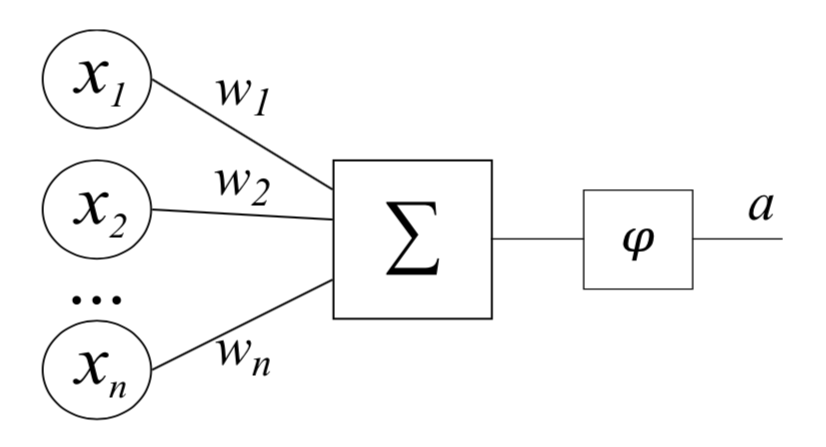
\includegraphics[width=0.7\textwidth]{fig/net}
\label{net}
\end{figure}


МакКаллок и Питтс предложили также метод объединения отдельных нейронов в
искусственные нейронные сети. Для этого выходные сигналы нейрона передаются на вход следующему нейрону \ref{qwe}. Нейронная сеть состоит из нескольких слоев, на каждом из которых может находиться несколько нейронов. Слои делятся на входные выходные и скрытные слои.
\begin{figure}[htbp]
\centering
\caption{Искусственная нейронная сеть}
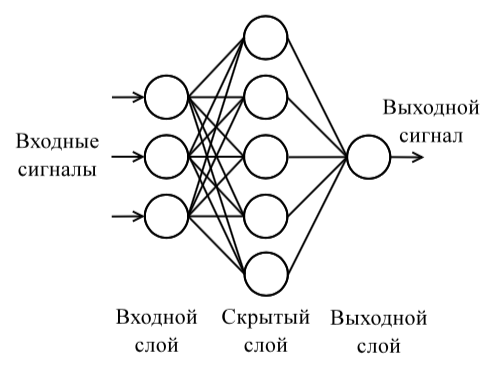
\includegraphics[width=0.7\textwidth]{fig/qwe}
\label{net}
\end{figure}

Однозначного определения, что такое глубокая нейронная сеть, не существует, но принято считать, что это сеть, которая содержит больше одного скрытого слоя.

Далее будут рассмотрены некоторые модели нейронны сетей.

\subsubsection{Рекуррентные нейронные сети }
\begin{figure}[htbp]
\centering
\caption{Рекуррентная нейронная сеть }
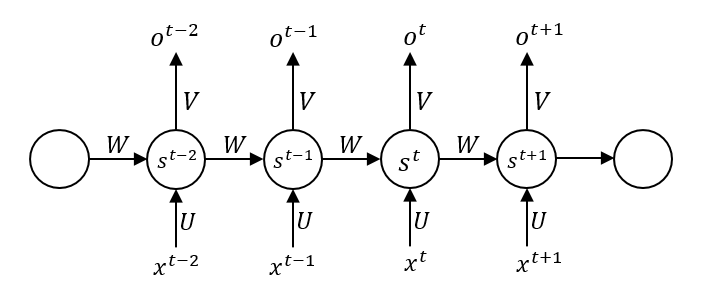
\includegraphics[width=0.7\textwidth]{fig/hzZ4m.png}
\end{figure}

Рекуррентные нейронные сети (Recurrent neural networks, RNN) были разработаны в 80 годах прошлого века. Прхитектура таких сетей строится из узлов, каждый из которых соединён со всеми другими узлами. У каждого нейрона порог активации меняется со временем и является вещественным числом. Каждое соединение имеет переменный вещественный вес. Узлы разделяются на входные, выходные и скрытые. 

В отличие от многослойных перцептронов, рекуррентные сети могут использовать свою внутреннюю память для обработки последовательностей произвольной длины. Поэтому сети RNN применимы в таких задачах, где нечто целостное разбито на сегменты, например: распознавание рукописного текста или распознавание речи. Было предложено много различных архитектурных решений для рекуррентных сетей.



\subsubsection{Свёрточные нейронные сети}

\begin{figure}[htbp]
\centering
\caption{Сверточная нейронная сеть}

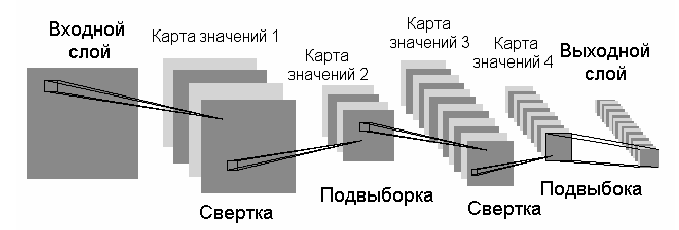
\includegraphics[width=0.9\textwidth]{fig/cnn}
\end{figure}

Свёрточные нейронные сети (convolutional neural networks, CNN)  отличаются от других сетей. Они используются в основном для обработки изображений. СНС чередует слои свертки и субдискретизации, а на выходе имеет несколько полносвязных слоев. Типичным способом применения CNN является классификация изображений. Такие сети обычно используют «сканер», не обрабатывающий все данные за один раз. Входные данные передаются через свёрточные слои, в которых не все узлы соединены между собой. Вместо этого каждый узел соединен только со своими ближайшими соседями. Эти слои имеют свойство сжиматься с глубиной, причём обычно они уменьшаются на какой-нибудь из делителей количества входных данных, часто используются степени двойки. 

Слой свертки и слой субдискретизации чередуясь между собой, формируют входной вектор признаков для многослойного персептрона.

\subsubsection{Генеративные состязательные сети}

\begin{figure}[htbp]
\centering
\caption{Генеративно состязательная сеть}
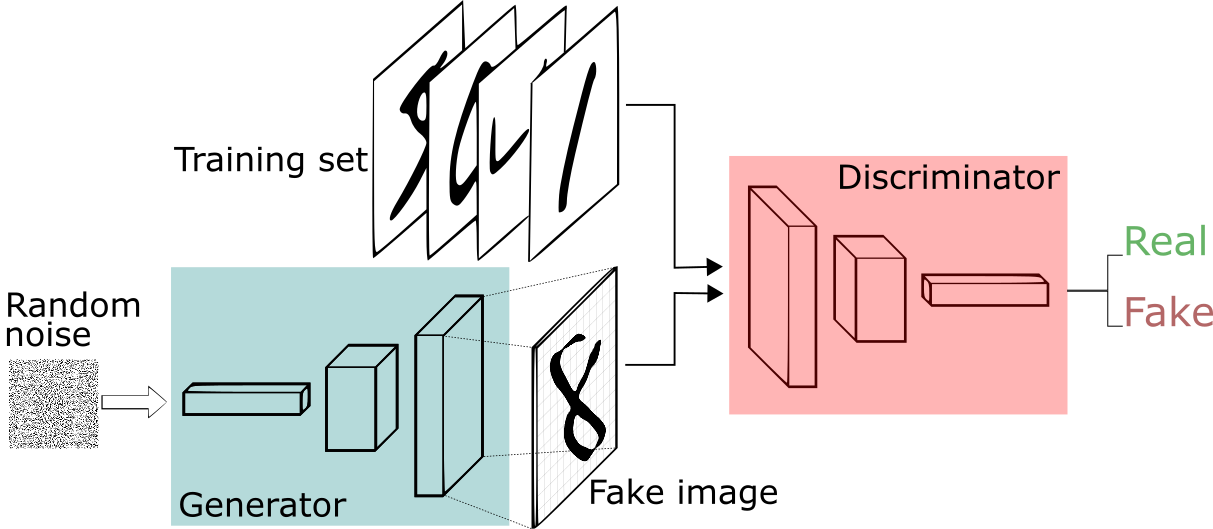
\includegraphics[width=0.9\textwidth]{fig/GANs.png}
\end{figure}

Генеративные состязательные сети (Generative adversarial networks, GAN) принадлежат другому семейству нейросетей. По сути, это две сети, работающие вместе. GAN состоит из любых двух сетей, где одна из сетей генерирует данные (“генератор”), а вторая - анализирует (“дискриминатор”). Дискриминатор получает на вход или обучающие данные, или сгенерированные первой сетью. То, насколько точно дискриминатор сможет определить источник данных, служит потом для оценки ошибок генератора. Таким образом, происходит своего рода соревнование, где дискриминатор учится лучше отличать реальные данные от сгенерированных, а генератор стремится стать менее предсказуемым для дискриминатора. Это работает отчасти потому, что даже сложные изображения с большим количеством шума в конце концов становятся предсказуемыми, но сгенерированные данные, мало отличающиеся от реальных, сложнее научиться отличать. GAN достаточно сложно обучить, так как задача здесь - не просто обучить две сети, но и соблюдать необходимый баланс между ними. Если одна из частей (генератор или дискриминатор) станет намного лучше другой, то GAN никогда не будет сходиться.


\subsubsection{Долгая краткосрочная память}
\begin{figure}[htbp]
\centering
\caption{Долгая краткосрочная память}
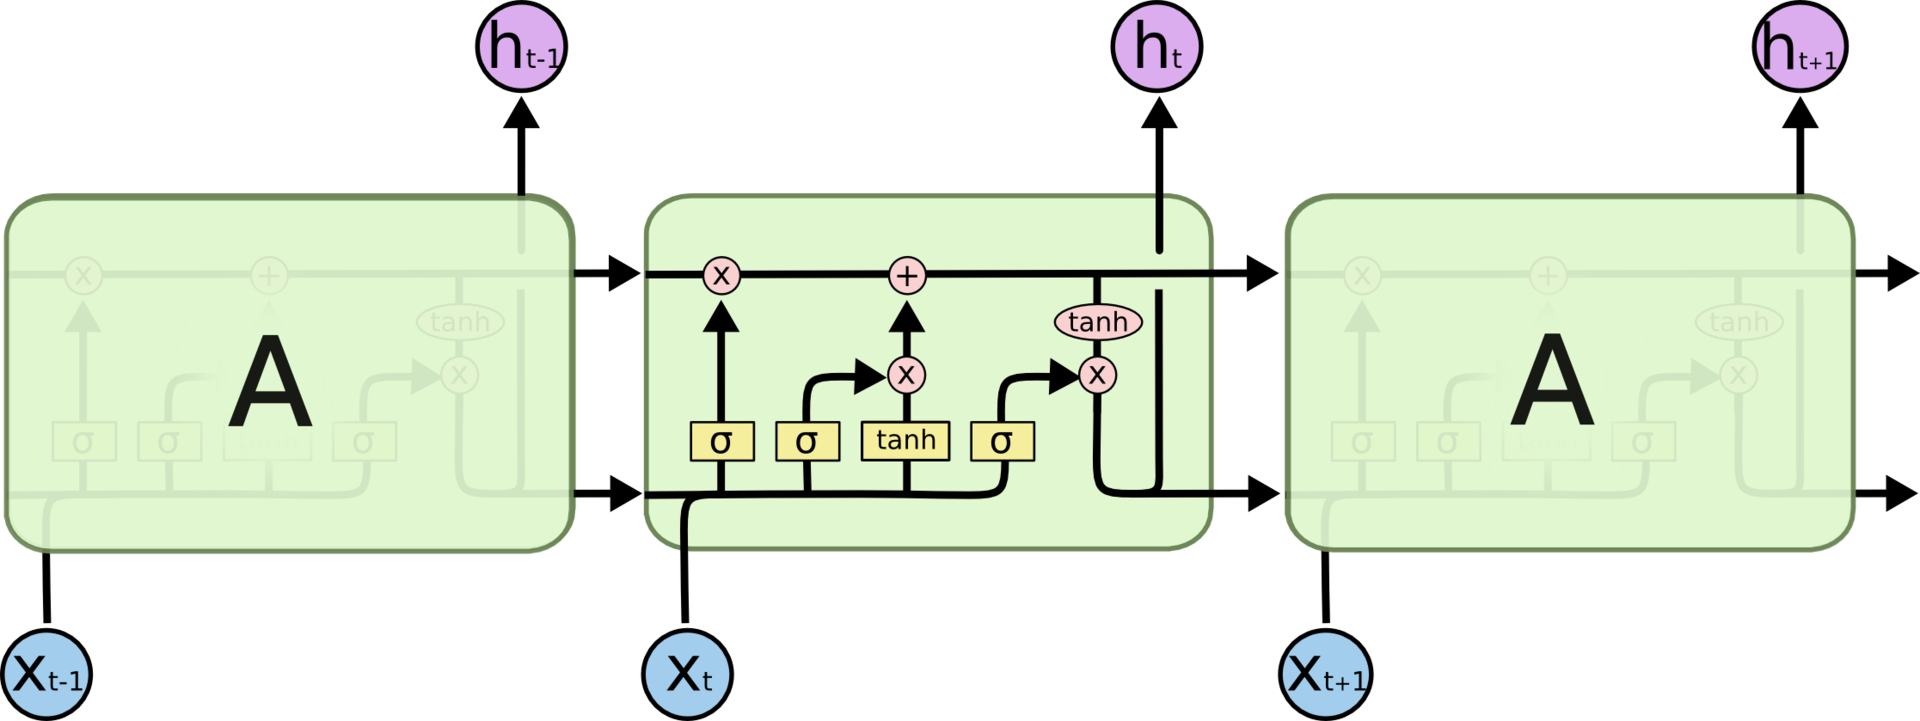
\includegraphics[width=0.7\textwidth]{fig/lstm}
\end{figure}
Долгая краткосрочная память (Long short term memory, LSTM) - попытка побороть проблему взрывного градиента, используя фильтры и блоки памяти. Эта идея пришла, скорее, из области схемотехники, а не биологии. У каждого нейрона есть три фильтра: входной фильтр, выходной фильтр и фильтр забывания. Задача этих фильтров - сохранять информацию, останавливая и возобновляя ее поток. Входной фильтр определяет количество информации с предыдущего шага, которое будет храниться в блоке памяти. Выходной фильтр занят тем, что определяет, сколько информации о текущем состоянии узла получит следующий слой. Наличие фильтра забывания на первый взгляд кажется странным, но иногда забывать оказывается полезно: если нейросеть запоминает книгу, в начале новой главы может быть необходимо забыть некоторых героев из предыдущей. Показано, что LSTM могут обучаться действительно сложным последовательностям, например, подражать Шекспиру или сочинять простую музыку. Стоит отметить, что так как каждый фильтр хранит свой вес относительно предыдущего нейрона, такие сети достаточно ресурсоемкости. Также существуют, двунаправленные LSTM. Разница лишь в том, что эти нейросети связаны не только с прошлым, но и с будущим.

\subsubsection{Сети прямого распространения}
\begin{figure}[htbp]
\centering
\caption{Сети прямого распространения}
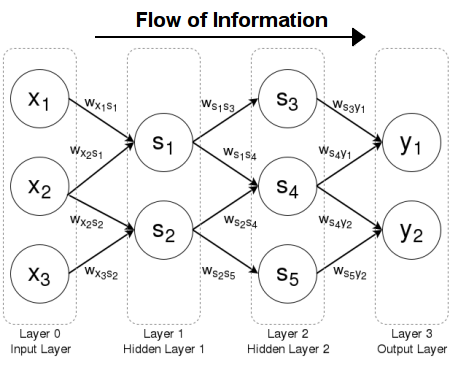
\includegraphics[width=0.7\textwidth]{fig/fnn}
\end{figure}

Сети прямого распространения (Feed forward neural networks, FF or FFNN) первая и самая простая нейронная сеть. Она передает информацию от входа к выходу без циклов. Нейроны одного слоя между собой не связаны, при этом каждый нейрон этого слоя связан с каждым нейроном соседнего слоя. FFNN обычно обучают методом обратного распространения ошибки, подавая модели на вход пары входных и ожидаемых выходных данных. На практике использование сетей прямого распространения ограничено, и чаще они используются совместно с другими сетями.
FFNN с радиально-базисной функцией в качестве функции активации называются сети радиально-базисных функций (radial basis function, RBF).

\subsubsection{Нейронная сеть Хопфилда}
\begin{figure}[htbp]
\centering
\caption{Нейронная сеть Хопфилда}
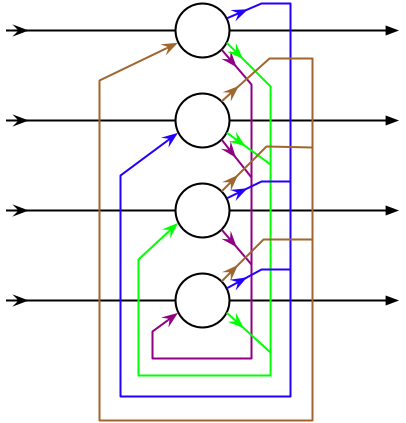
\includegraphics[width=0.7\textwidth]{fig/Hopfield}
\end{figure}
Нейронная сеть Хопфилда - полносвязная сеть, это означает, что каждый нейрон соединен с каждым. Сеть Хопфилда является сетью с обратной связью, что означает, что ее выходы перенаправляются на входные данные. Количество узлов входов равно количеству выходов сети. Кроме того, каждый из нейронов имеет двоичное состояние или значение активации, обычно представленное как 1 или -1. Состояние каждого узла обычно сходится, это означает, что состояние каждого узла становится фиксированным после определенного количества обновлений.

\subsubsection{Ограниченная машина Больцмана}
\begin{figure}[htbp]
\centering
\caption{Ограниченная машина Больцмана}
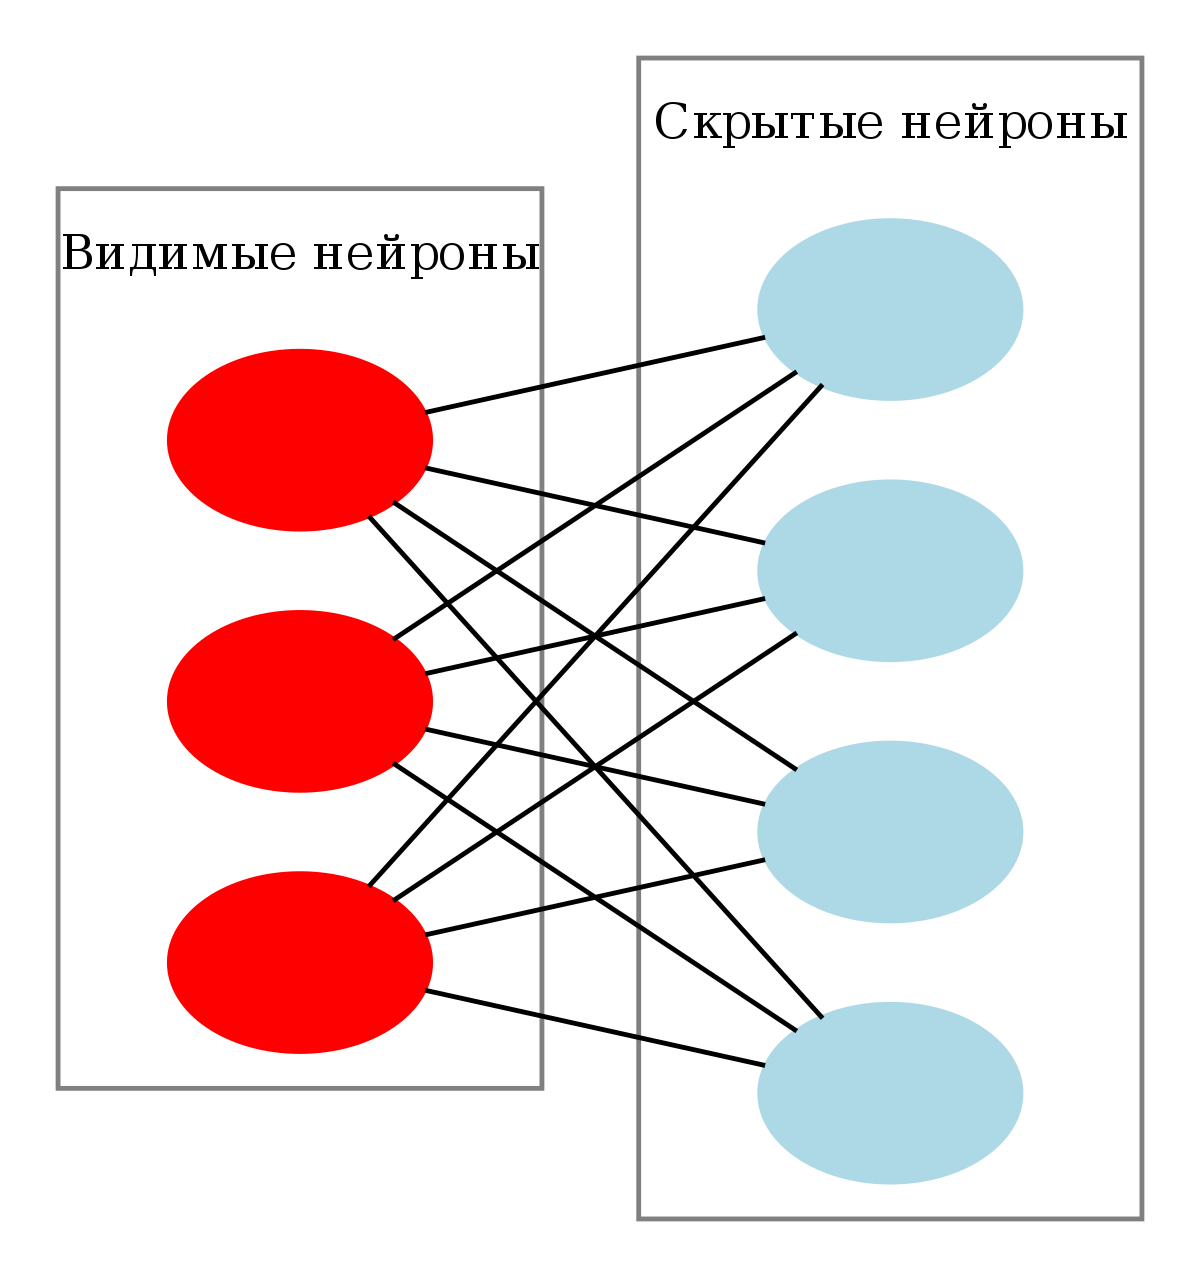
\includegraphics[width=0.7\textwidth]{fig/vg.png.png}
\end{figure}
Ограниченная машина Больцмана (Restricted Boltzmann machine, RBM) - вид генеративной стохастической нейронной сети, которая определяет распределение вероятности на входных образцах данных. В них каждый нейрон не связан с каждым, а только каждая группа нейронов соединена с другими группами. Входные нейроны не связаны между собой, нет соединений и между скрытыми нейронами. RBM можно обучать так же, как и сети прямого распространения, за небольшим отличием: вместо передачи данных вперед и последующего обратного распространения ошибки, данные передаются вперед и назад, а затем применяется прямое и обратное распространение.

\subsubsection{Автоэнкодеры}
\begin{figure}[htbp]
\centering
\caption{Автоэнкодеры}
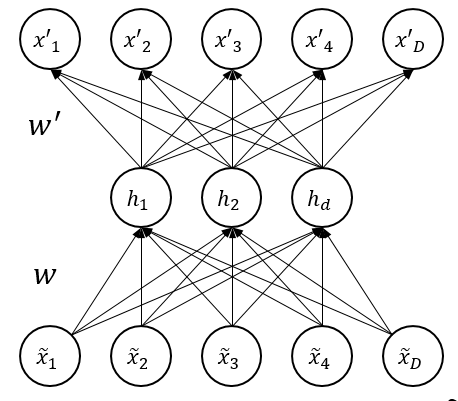
\includegraphics[width=0.7\textwidth]{fig/AE}
\end{figure}
Автоэнкодеры (Autoencoders, AE) - подобны сетям прямого распространения. Основная идея автоэнкодеров - автоматическое кодирование информации, отсюда и название. Сеть напоминает по форме песочные часы, так как скрытый слой меньше, чем входной и выходной; к тому же она симметрична относительно средних слоев (одного или двух, в зависимости от четности/нечетности общего количества слоев). Самый маленьких слой почти всегда средний, в нем информация максимально сжата. Все, что расположено до середины — кодирующая часть, выше середины — декодирующая, а в середине - код. AE обучают методом обратного распространения ошибки, подавая входные данные и задавая ошибку равной разницу между входом и выходом. AE можно построить симметричными и с точки зрения весов, выставляя кодирующие веса равными декодирующим.


\subsubsection{Глубокие сети доверия}
\begin{figure}[htbp]
	\centering
			\caption{Глубокая сеть доверия}
	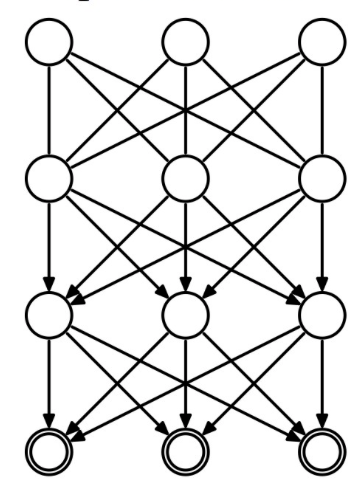
\includegraphics[width=0.7\textwidth]{fig/DBN}
\end{figure}
Глубокие сети доверия (Deep belief networks, DBN) - сети, представляющие собой композицию нескольких ограниченных машин Больцмана. Такие сети показали себя эффективно обучаемыми одна за другой, когда каждая сеть должна научиться кодировать предыдущую. Этот метод также называют “жадное обучение”, он заключается в принятии оптимального на данный момент решение, чтобы получить подходящий, но, возможно, не оптимальный результат. Глубокие сети доверия могут обучаться методами contrastive divergence или обратным распространением ошибки и учатся представлять данные в виде вероятностной модели, в точности как ограниченные машины Больцмана. Один раз обученную и приведенную к стационарному состоянию модель можно использовать для генерации новых данных.




\subsubsection{Нейронные эхо-сети}
\begin{figure}[htbp]
	\centering
			\caption{Нейронные эхо-сети}
	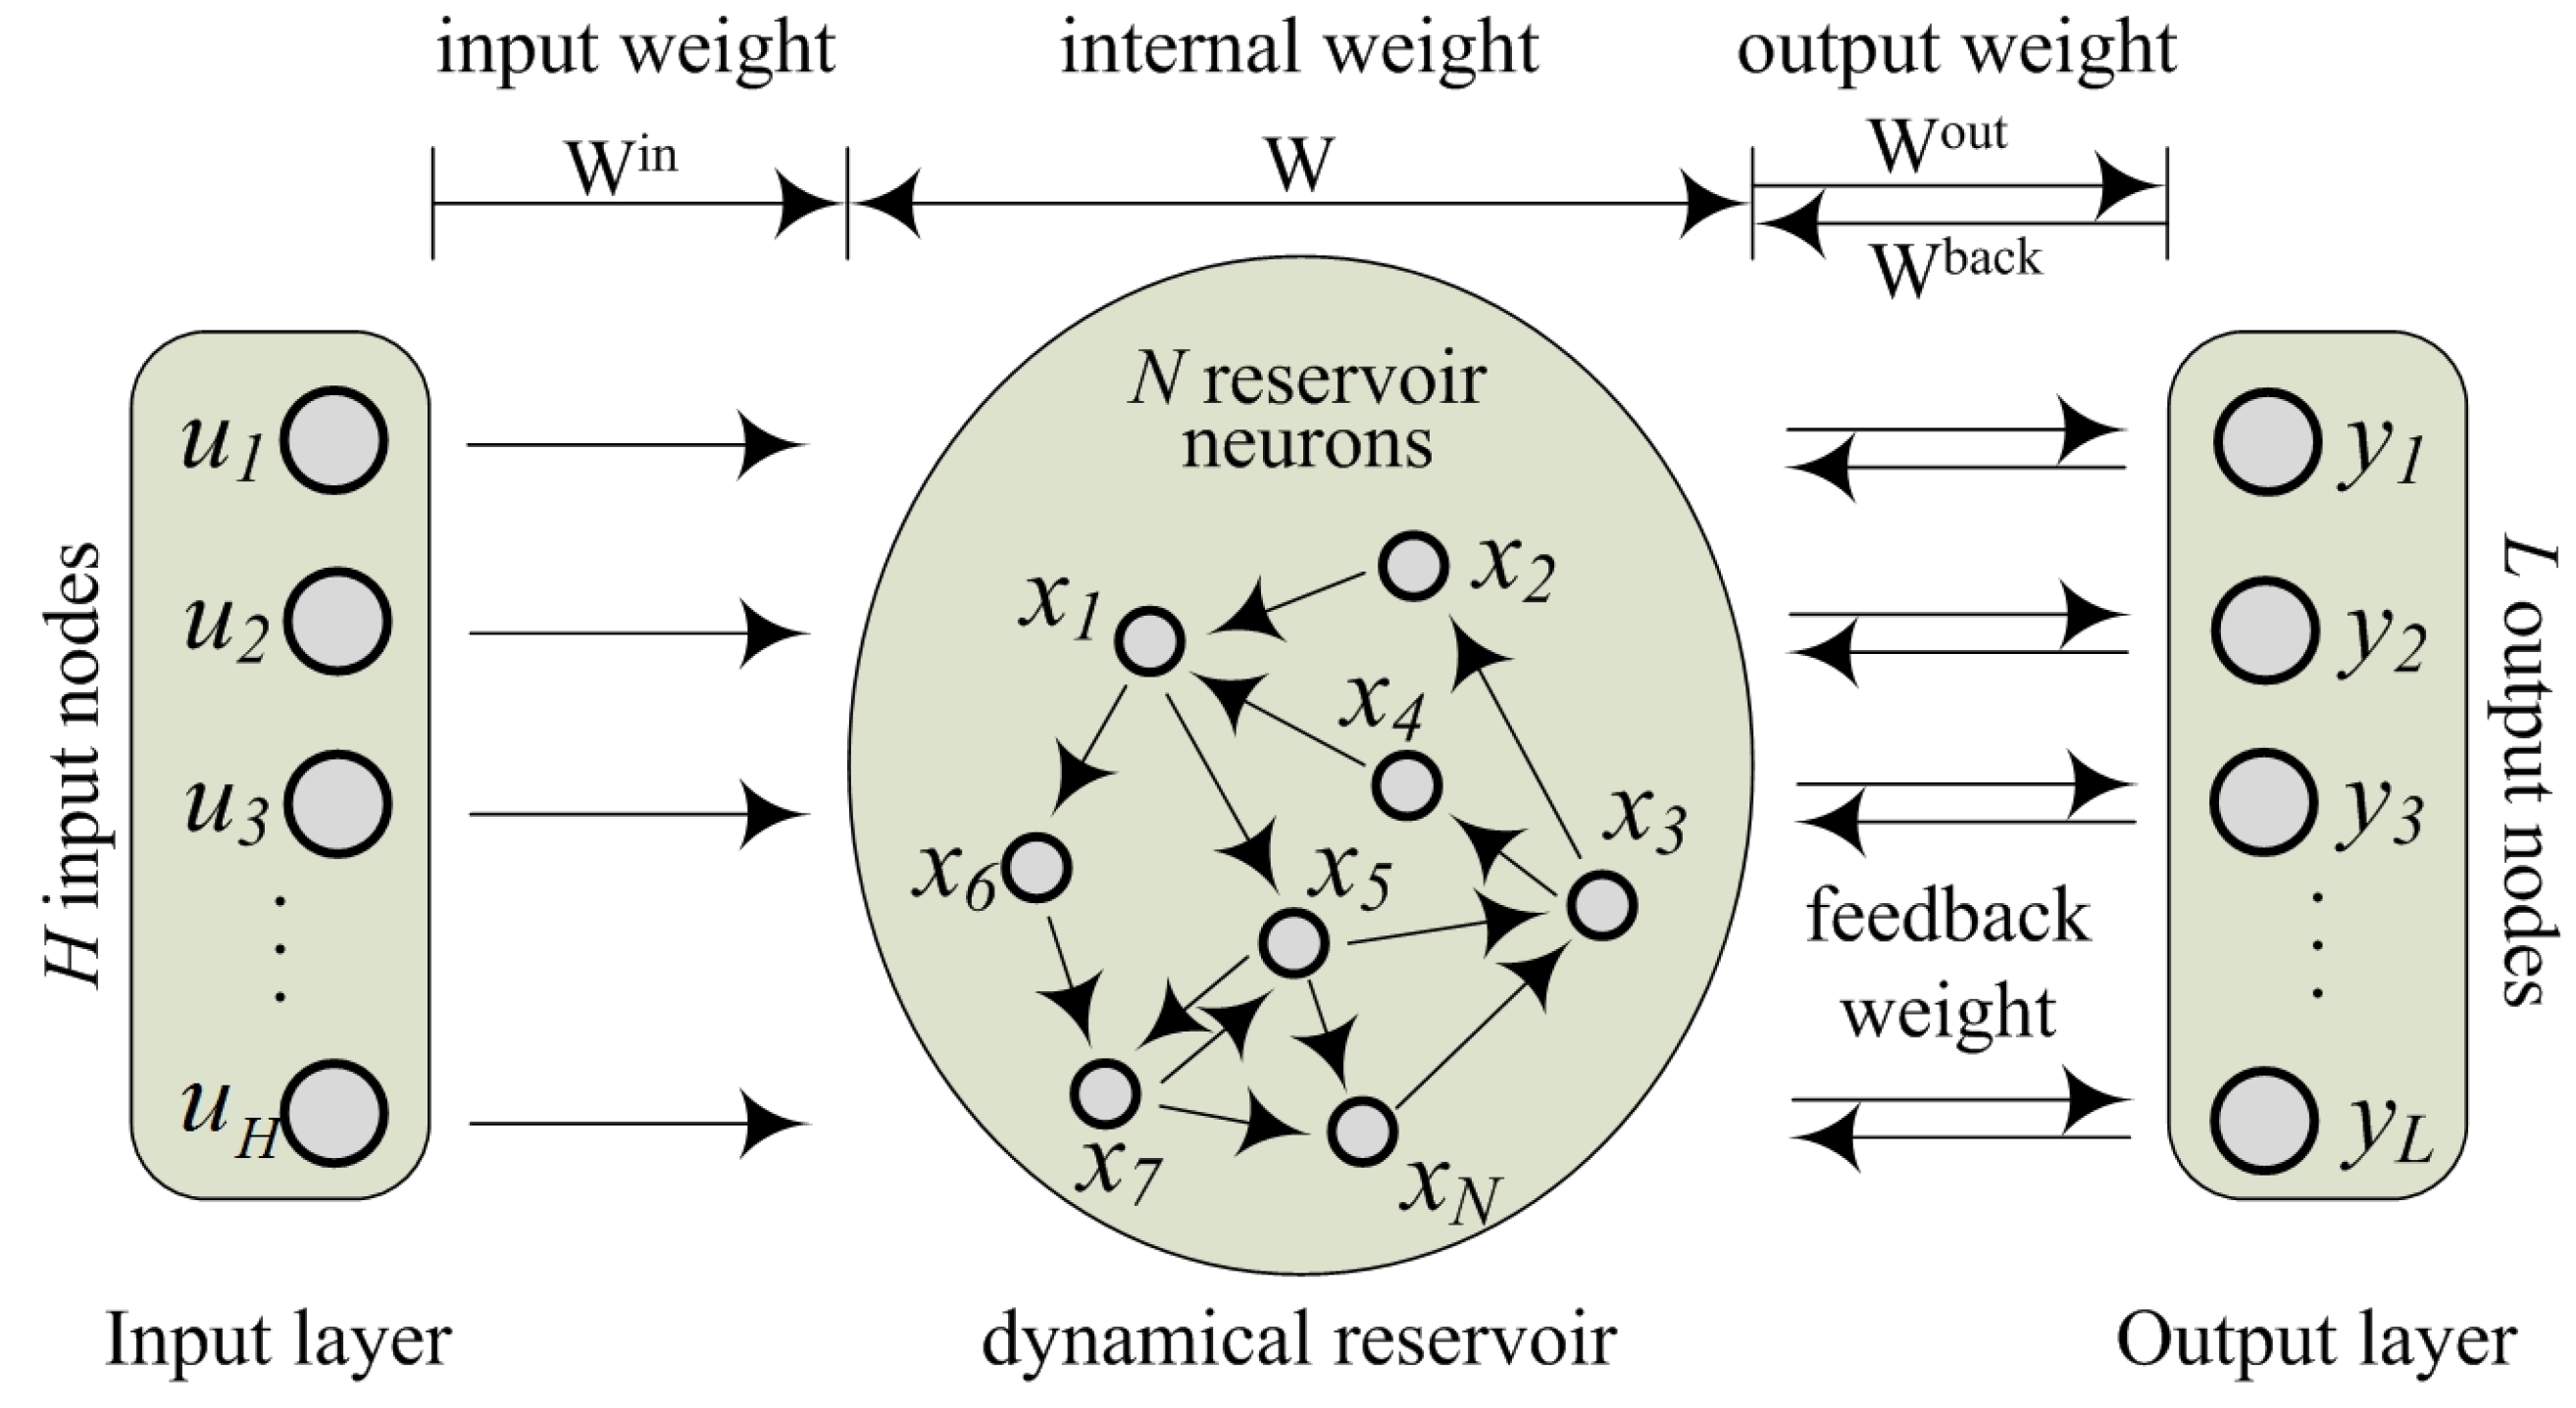
\includegraphics[width=0.7\textwidth]{fig/ESN.png}
\end{figure}
Нейронные эхо-сети (Echo state networks, ESN) — еще один вид рекуррентных нейросетей. Они выделяются тем, что связи между нейронами в них случайны, не организованы в аккуратные слои, и обучаются они по-другому. Вместо подачи на вход данных и обратного распространения ошибки, мы передаем данные, обновляем состояния нейронов и в течение некоторого времени следим за выходными данными. Входной и выходной слои играют нестандартную роль, так как входной слой служит для инициализации системы, а выходной слой - в качестве наблюдателя за порядком активации нейронов, который проявляется со временем. Во время обучения изменяются связи только между наблюдателем и скрытыми слоями.







\section{Существующие лабораторные работы}

Институт глубокого обучения NVIDIA (DLI) предлагает пройти практические занятия для разработчиков, специалистов по обработке данных, которые решают сложные задачи с применением технологии глубокого обучения. NVIDIA предлагает узнать о современных техниках проектирования, тренировки и интеграции алгоритмов машинного обучения в самые разные приложения. Курс предлагает научиться работать с популярными фреймворками с открытым исходным кодом и новейшими платформами глубокого обучения с ускорением на NVIDIA GPU.

NVIDIA предлагает следующие области \cite{NVIDIA}:
\begin{itemize}
\item глубокое обучение в области компьютерного зрения;
\item глубокое обучения для работы с разными типами данных;
\item глубокое обучение для обработки естественных языков;
\item глубокое обучение в области геномики;
\item глубокое обучение для анализа медицинских изображений;
\item восприятие окружающего мира у беспилотных автомобилей;
\item создание цифрового контента с помощью генеративно-состязательных сетей и автоэнкодеров;
\item основы ускоренных вычислений с CUDA C/C++;
\item основы ускоренных вычислений с OpenACC;
\item глубокое обучения для разработки стратегии торгового финансирования;
\item глубокое обучение для анализа полномасштабного видео.
\end{itemize}

Эти лабораторные работы не подходят для изучения в рамках университетской программы, так как только первые три из них  бесплатные, на прохождение каждой из них дается полтора часа, и основываются на  веб-приложение DIGITS. DIGITS (the Deep Learning GPU Training System) - это веб-приложение для обучения глубоким учебным моделям. В настоящее время поддерживаемые структуры: Caffe, Torch и Tensorflow. 